\documentclass[aspectratio=169,11pt]{beamer}

\usepackage[utf8]{inputenc}
\usepackage[T1]{fontenc}
\usepackage{lmodern}
\usepackage{amsmath,amssymb}
\usepackage{booktabs}
\usepackage{tikz}
\usepackage{pgfplots}
\pgfplotsset{compat=1.18}
\usetikzlibrary{arrows.meta,positioning,shapes.geometric,calc}

\usetheme{Madrid}
\setbeamertemplate{navigation symbols}{}
\setbeamertemplate{footline}[frame number]

\definecolor{deepblue}{RGB}{33,82,135}
\definecolor{softblue}{RGB}{84,145,196}
\definecolor{softgreen}{RGB}{95,166,119}
\definecolor{softorange}{RGB}{232,148,82}
\definecolor{softred}{RGB}{199,85,85}
\definecolor{darkgray}{RGB}{65,65,65}
\setbeamercolor{structure}{fg=deepblue}
\setbeamercolor{frametitle}{fg=white,bg=deepblue}
\setbeamercolor{title}{fg=white,bg=deepblue}

\title[Bűnözési gyakoriság modellezése]{Bűnözési gyakoriság modellezése}
\subtitle{Sztochasztikus és gépi tanulási módszerek alkalmazása}
\author{Győrfi Enikő}
\institute{Eötvös Loránd Tudományegyetem}
\date{Szakdolgozatvédés, 2026}

\newcommand{\smallnote}[1]{\vspace{0.12cm}{\scriptsize\color{darkgray}#1}}
\newcommand{\heatcell}[4]{% x y intensity text
  \pgfmathsetmacro{\shade}{15 + 75*#3}
  \fill[softblue!\shade!white] (#1,#2) rectangle ++(0.55,0.42);
  \node[font=\tiny] at ($(#1,#2)+(0.275,0.21)$) {#4};}
\newcommand{\heatcellg}[4]{% green heatmap
  \pgfmathsetmacro{\shade}{15 + 75*#3}
  \fill[softgreen!\shade!white] (#1,#2) rectangle ++(0.52,0.34);
  \node[font=\tiny] at ($(#1,#2)+(0.26,0.17)$) {#4};}

\begin{document}

% 1
\begin{frame}
  \titlepage
\end{frame}
 %2
\begin{frame}{Motiváció}

\centering
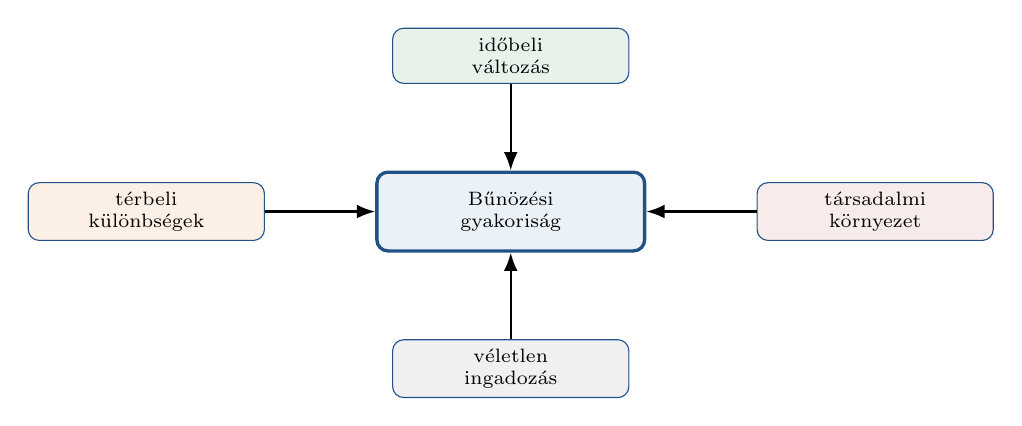
\begin{tikzpicture}[
  every node/.style={font=\scriptsize},
  node distance=0.8cm
]

% Központi elem
\node[
  draw=deepblue,
  very thick,
  rounded corners,
  fill=softblue!12,
  minimum width=3.4cm,
  minimum height=1.0cm,
  align=center
] (crime) {Bűnözési\\gyakoriság};

% Környező tényezők
\node[
  draw=deepblue,
  rounded corners,
  fill=softgreen!15,
  above=1.1cm of crime,
  minimum width=3.0cm,
  minimum height=0.7cm,
  align=center
] (time) {időbeli\\változás};

\node[
  draw=deepblue,
  rounded corners,
  fill=softorange!15,
  left=1.4cm of crime,
  minimum width=3.0cm,
  minimum height=0.7cm,
  align=center
] (space) {térbeli\\különbségek};

\node[
  draw=deepblue,
  rounded corners,
  fill=softred!12,
  right=1.4cm of crime,
  minimum width=3.0cm,
  minimum height=0.7cm,
  align=center
] (society) {társadalmi\\környezet};

\node[
  draw=deepblue,
  rounded corners,
  fill=gray!12,
  below=1.1cm of crime,
  minimum width=3.0cm,
  minimum height=0.7cm,
  align=center
] (random) {véletlen\\ingadozás};

% Nyilak
\draw[-Latex,thick] (time) -- (crime);
\draw[-Latex,thick] (space) -- (crime);
\draw[-Latex,thick] (society) -- (crime);
\draw[-Latex,thick] (random) -- (crime);

\end{tikzpicture}

\vspace{0.45cm}

\begin{center}
\begin{minipage}{0.55\textwidth}
\begin{block}{Modellezési kérdés}
\centering
Hogyan jelezhető előre a bűnözés alakulása?
\end{block}
\end{minipage}
\end{center}

\end{frame}

% 3
\begin{frame}{Elméleti háttér: geometriai Brown-mozgás}

    \begin{columns}[T]

        % BAL OSZLOP: Modellegyenletek (A kép alapján)
        \begin{column}{0.53\textwidth}

            \begin{block}{Sztochasztikus differenciálegyenlet}
                \vspace{-0.2cm}
                \[ dS(t) = \underbrace{\mu S(t)dt}_{\text{drift}} + \underbrace{\sigma S(t)dB(t)}_{\text{diffúzió}} \]
            \end{block}

            \vspace{0.1cm}

            \begin{block}{Explicit megoldás}
                \vspace{-0.4cm}
                \[ S(t) = S(0) \exp\left( \left( \mu - \frac{1}{2}\sigma^2 \right)t + \sigma B(t) \right) \]
            \end{block}

        \end{column}

        % JOBB OSZLOP: Elméleti tulajdonságok (Ábra helyett)
        \begin{column}{0.45\textwidth}

            \begin{block}{A folyamat tulajdonságai}
                \small
                \begin{itemize}
                    \item \textbf{Szigorú pozitivitás:}\\ Az exponenciális alak miatt garantáltan $S(t) > 0$.
                    \vspace{0.2cm}
                    \item \textbf{Lognormális eloszlás:}\\ Minden $t > 0$ esetén $S(t)$ lognormális eloszlást követ.
                    \vspace{0.2cm}

                    \item \textbf{Várható érték:}\\ $\mathbb{E}[S(t)] = S(0)\exp(\mu t)$
                    \vspace{0.2cm}
                    \item \textbf{Szórásnégyzet:}\\ $Var[S(t)] = S^2(0)e^{2\mu t}(e^{\sigma^2 t} - 1)$
                \end{itemize}
            \end{block}

        \end{column}

    \end{columns}

\end{frame}

% 5
\begin{frame}{Elméleti háttér II: Random Forest}
\begin{columns}[T]

\begin{column}{0.57\textwidth}
\centering
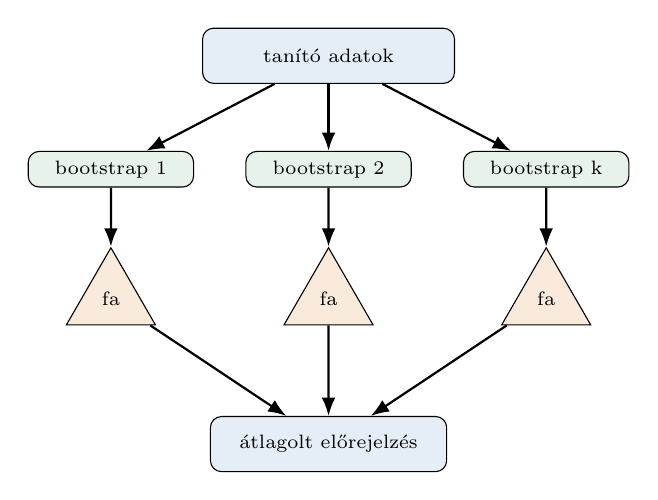
\begin{tikzpicture}[node distance=0.8cm, every node/.style={font=\scriptsize}]
  \node[draw,rounded corners,fill=softblue!15,minimum width=3.2cm,minimum height=0.7cm] (d) {tanító adatok};

  \node[draw,rounded corners,fill=softgreen!15,below left=0.85cm and 0.1cm of d,minimum width=2.1cm] (b1) {bootstrap 1};
  \node[draw,rounded corners,fill=softgreen!15,below=0.85cm of d,minimum width=2.1cm] (b2) {bootstrap 2};
  \node[draw,rounded corners,fill=softgreen!15,below right=0.85cm and 0.1cm of d,minimum width=2.1cm] (b3) {bootstrap k};

  \node[draw,regular polygon,regular polygon sides=3,fill=softorange!20,below=0.75cm of b1,minimum size=1.1cm] (t1) {fa};
  \node[draw,regular polygon,regular polygon sides=3,fill=softorange!20,below=0.75cm of b2,minimum size=1.1cm] (t2) {fa};
  \node[draw,regular polygon,regular polygon sides=3,fill=softorange!20,below=0.75cm of b3,minimum size=1.1cm] (t3) {fa};

  \node[draw,rounded corners,fill=softblue!15,below=1.15cm of t2,minimum width=3.0cm,minimum height=0.7cm] (avg) {átlagolt előrejelzés};

  \foreach \a/\b in {d/b1,d/b2,d/b3,b1/t1,b2/t2,b3/t3,t1/avg,t2/avg,t3/avg}{
    \draw[-Latex,thick] (\a) -- (\b);
  }
\end{tikzpicture}
\end{column}

\begin{column}{0.36\textwidth}
\vspace{0.25cm}

\begin{block}{Működése}
\begin{itemize}
  \item bootstrap minták,
  \item több döntési fa,
  \item véletlen változóválasztás,
  \item átlagolt becslés.
\end{itemize}
\end{block}

\vspace{0.25cm}

\begin{block}{Előnye}
Csökkenti a fák korrelációját és ezáltal a modell varianciáját.
\end{block}

\end{column}
\end{columns}

\end{frame}

% 3
\begin{frame}{Adatok: Chicago bűnözési adatai}
\begin{columns}[T]
\begin{column}{0.48\textwidth}
\centering

\includegraphics[width=1\textwidth]{major_crimes_chicago.png}
\end{column}
\begin{column}{0.48\textwidth}
\begin{block}{Felhasznált felbontások}
\begin{itemize}
  \item \textbf{2001--2025}: több millió rekord
  \item \textbf{havi idősor}: rendőrségi körzetek
  \item \textbf{éves panel}: Community Area szint
  \item \textbf{ACS}: társadalmi-demográfiai adatok
\end{itemize}
\end{block}
\vspace{0.35cm}
\begin{block}{Kiértékelés}
\begin{itemize}
  \item RMSE, MAE, MAPE, Accuracy
  \item típusonként: WMAPE
\end{itemize}
\end{block}
\end{column}
\end{columns}
\end{frame}


% 4

\begin{frame}{Modellezési terv}

\centering
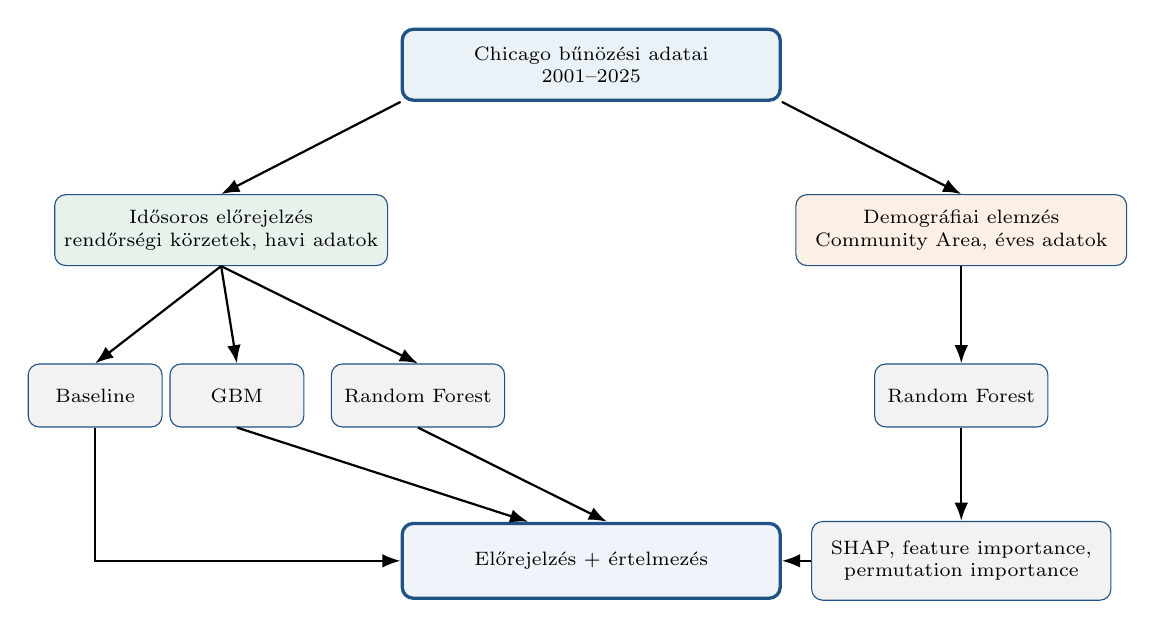
\begin{tikzpicture}[
  every node/.style={font=\scriptsize},
  >=Latex
]

% --- Csomópontok ---

% Felső fő csomópont
\node[
  draw=deepblue,
  very thick,
  rounded corners,
  fill=softblue!12,
  minimum width=4.8cm,
  minimum height=0.9cm,
  align=center
] (data) at (0,0) {Chicago bűnözési adatai\\2001--2025};

% Bal ág
\node[
  draw=deepblue,
  rounded corners,
  fill=softgreen!15,
  minimum width=4.2cm,
  minimum height=0.9cm,
  align=center
] (time) at (-4.7,-2.1) {Idősoros előrejelzés\\rendőrségi körzetek, havi adatok};

% Jobb ág
\node[
  draw=deepblue,
  rounded corners,
  fill=softorange!15,
  minimum width=4.2cm,
  minimum height=0.9cm,
  align=center
] (demo) at (4.7,-2.1) {Demográfiai elemzés\\Community Area, éves adatok};

% Bal oldali modellek
\node[
  draw=deepblue,
  rounded corners,
  fill=gray!10,
  minimum width=1.7cm,
  minimum height=0.8cm,
  align=center
] (base) at (-6.3,-4.2) {Baseline};

\node[
  draw=deepblue,
  rounded corners,
  fill=gray!10,
  minimum width=1.7cm,
  minimum height=0.8cm,
  align=center
] (gbm) at (-4.5,-4.2) {GBM};

\node[
  draw=deepblue,
  rounded corners,
  fill=gray!10,
  minimum width=2.2cm,
  minimum height=0.8cm,
  align=center
] (rf) at (-2.2,-4.2) {Random Forest};

% Jobb oldali modellek
\node[
  draw=deepblue,
  rounded corners,
  fill=gray!10,
  minimum width=2.2cm,
  minimum height=0.8cm,
  align=center
] (rfdemo) at (4.7,-4.2) {Random Forest};

\node[
  draw=deepblue,
  rounded corners,
  fill=gray!10,
  minimum width=3.8cm,
  minimum height=1.0cm,
  align=center
] (interpret) at (4.7,-6.3) {SHAP, feature importance,\\permutation importance};

% Alsó közös cél
\node[
  draw=deepblue,
  very thick,
  rounded corners,
  fill=softblue!10,
  minimum width=4.8cm,
  minimum height=0.95cm,
  align=center
] (goal) at (0,-6.3) {Előrejelzés + értelmezés};


% --- Nyilak és összeköttetések ---

% Nyilak felülről a két fő ághoz
\draw[->,thick] (data.south west) -- (time.north);
\draw[->,thick] (data.south east) -- (demo.north);

% Bal ág lefelé a 3 modellhez
\draw[->,thick] (time.south) -- (base.north);
\draw[->,thick] (time.south) -- (gbm.north);
\draw[->,thick] (time.south) -- (rf.north);

% Jobb ág lefelé a modellhez és a SHAP-hoz
\draw[->,thick] (demo.south) -- (rfdemo.north);
\draw[->,thick] (rfdemo.south) -- (interpret.north);


% --- ÚJ, SPECIFIKUS NYÍLSTÍLUSOK A CÉL DOBOZHOZ ---

% 1. Baseline -> Derékszögben törő nyíl a cél doboz BAL oldalába
\draw[->,thick] (base.south) |- (goal.west);

% 2. GBM -> FERDE nyíl a cél doboz tetejére (balra tolva)
\draw[->,thick] (gbm.south) -- ([xshift=-0.8cm]goal.north);

% 3. Idősoros Random Forest -> Enyhén ferde nyíl a cél doboz tetejére (középtájt)
\draw[->,thick] (rf.south) -- ([xshift=0.2cm]goal.north);

% 4. SHAP (Értelmezés) -> Vízszintes egyenes nyíl a cél doboz JOBB oldalába
\draw[->,thick] (interpret.west) -- (goal.east);

\end{tikzpicture}

\end{frame}
% 6
% 7
\begin{frame}{Baseline modell: 3 hónapos mozgóátlag}
\begin{columns}[T]
\begin{column}{0.52\textwidth}
\centering
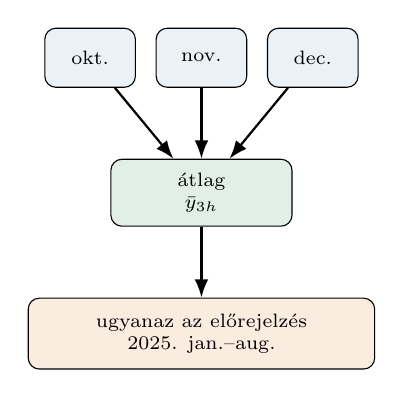
\begin{tikzpicture}[every node/.style={font=\scriptsize}]
  \node[draw,rounded corners,fill=softblue!12,minimum width=1.15cm,minimum height=0.75cm] (oct) at (0,0) {okt.};
  \node[draw,rounded corners,fill=softblue!12,minimum width=1.15cm,minimum height=0.75cm,right=0.25cm of oct] (nov) {nov.};
  \node[draw,rounded corners,fill=softblue!12,minimum width=1.15cm,minimum height=0.75cm,right=0.25cm of nov] (dec) {dec.};
  \node[draw,rounded corners,fill=softgreen!18,minimum width=2.3cm,minimum height=0.85cm,below=0.9cm of nov,align=center] (avg) {átlag\\$\bar y_{3h}$};
  \node[draw,rounded corners,fill=softorange!18,minimum width=4.4cm,minimum height=0.9cm,below=0.9cm of avg,align=center] (pred) {ugyanaz az előrejelzés\\2025. jan.--aug.};
  \draw[-Latex,thick] (oct) -- (avg);
  \draw[-Latex,thick] (nov) -- (avg);
  \draw[-Latex,thick] (dec) -- (avg);
  \draw[-Latex,thick] (avg) -- (pred);
\end{tikzpicture}
\vspace{0.35cm}

\begin{center}
\begin{tabular}{llll}
\toprule
RMSE & MAE & MAPE & Acc.\\
\midrule
3.19 & 2.51 & 8.81 & 91.19\\
\bottomrule
\end{tabular}
\end{center}
\end{column}
\begin{column}{0.44\textwidth}
\begin{block}{Miért kellett baseline?}
\begin{itemize}
  \item egyszerű viszonyítási alap,
  \item nem tanul paramétereket,
  \item csak a legutóbbi rövid távú szintet használja.
\end{itemize}
\end{block}
\vspace{0.2cm}
\begin{block}{Értelmezés}
A jó baseline-eredmény azt mutatja, hogy a bűnözési adatokban erős \textbf{rövid távú perzisztencia} van.
\end{block}

\end{column}
\end{columns}
\end{frame}

% 8
\begin{frame}{GBM modell: korrelált Brown-mozgások}
\begin{columns}[T]
\begin{column}{0.50\textwidth}
\begin{block}{Körzetenkénti modell}
\[
 dS_{i,t}=\mu_i S_{i,t}dt+\sigma_i S_{i,t}dW_{i,t}
\]
\[
 S_{i,t}=S_{i,0}\exp\!\left(\left(\mu_i-\frac{\sigma_i^2}{2}\right)t+\sigma_iW_{i,t}\right)
\]
\end{block}
\begin{itemize}
  \item $\mu_i$: hosszú távú trend,
  \item $\sigma_i$: volatilitás,
  \item $S_{i,0}$: 2024. decemberi érték.
\end{itemize}
\begin{block}{Lényeg}
A GBM nem determinisztikus predikció, hanem \textbf{lehetséges jövőbeli pályák} szimulációja.
\end{block}
\end{column}
\begin{column}{0.46\textwidth}
\centering
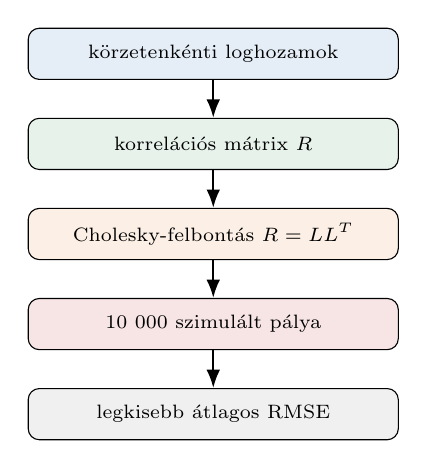
\begin{tikzpicture}[every node/.style={font=\scriptsize}]
  \node[draw,rounded corners,fill=softblue!15,minimum width=4.7cm,minimum height=0.65cm] (returns) {körzetenkénti loghozamok};
  \node[draw,rounded corners,fill=softgreen!15,below=0.48cm of returns,minimum width=4.7cm,minimum height=0.65cm] (corr) {korrelációs mátrix $R$};
  \node[draw,rounded corners,fill=softorange!15,below=0.48cm of corr,minimum width=4.7cm,minimum height=0.65cm] (chol) {Cholesky-felbontás $R=LL^T$};
  \node[draw,rounded corners,fill=softred!15,below=0.48cm of chol,minimum width=4.7cm,minimum height=0.65cm] (scen) {10 000 szimulált pálya};
  \node[draw,rounded corners,fill=gray!12,below=0.48cm of scen,minimum width=4.7cm,minimum height=0.65cm] (best) {legkisebb átlagos RMSE};
  \foreach \a/\b in {returns/corr,corr/chol,chol/scen,scen/best}{\draw[-Latex,thick] (\a) -- (\b);} 
\end{tikzpicture}
\vspace{0.2cm}

\end{column}
\end{columns}
\end{frame}

% 9



\begin{frame}{GBM modell eredményei hőtérképen}
\begin{columns}[T,onlytextwidth]

  \begin{column}{0.32\textwidth}
    \centering
    \includegraphics[
      width=0.9\textwidth,
      trim=0.3cm 0.2cm 0.4cm 0.2cm,
      clip
    ]{gbm_predicted_heatmap_2.png}

    \vspace{-0.5cm}
    {\scriptsize GBM előrejelzés}
  \end{column}

  \hspace{-0.2cm}

  \begin{column}{0.32\textwidth}
    \centering
    \includegraphics[
      width=0.9\textwidth,
      trim=0.3cm 0.2cm 0.4cm 0.2cm,
      clip
    ]{gbm_actual_heatmap_2.png}

    \vspace{-0.5cm}
    {\scriptsize Tényleges adatok}
  \end{column}

  \hspace{-0.2cm}

  \begin{column}{0.32\textwidth}
    \centering
    \includegraphics[
      width=0.9\textwidth,
      trim=0.3cm 0.2cm 0.4cm 0.2cm,
      clip
    ]{gbm_difference_heatmap_2.png}

    \vspace{-0.5cm}
    {\scriptsize Abszolút eltérés}
  \end{column}

\end{columns}

\vspace{0.2cm}

\centering
\begin{tabular}{rrrr}
\toprule
RMSE & MAE & MAPE & Accuracy\\
\midrule
3.34 & 2.64 & 8.93 & 91.07\\
\bottomrule
\end{tabular}

\vspace{0.1cm}

\end{frame}



% RF comparison slide
\begin{frame}{Két Random Forest modell}
\small
\begin{columns}[T]
\begin{column}{0.48\textwidth}
\begin{block}{Modell 1: lag feature-ök}
\begin{itemize}
  \item csak az előző hónapok értékei,
  \item legjobb változat: \textbf{2 lag},
  \item rövid távú múlt hatását méri.
\end{itemize}
\end{block}
\centering
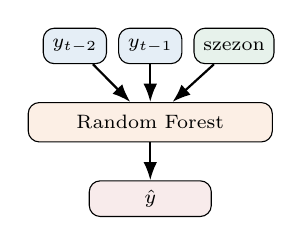
\begin{tikzpicture}[node distance=0.28cm, every node/.style={font=\scriptsize}]
  \node[draw,rounded corners,fill=softblue!15,minimum width=0.75cm,minimum height=0.45cm] (m2) {$y_{t-2}$};
  \node[draw,rounded corners,fill=softblue!15,right=0.14cm of m2,minimum width=0.75cm,minimum height=0.45cm] (m1) {$y_{t-1}$};
  \node[draw,rounded corners,fill=softgreen!15,right=0.14cm of m1,minimum width=0.95cm,minimum height=0.45cm] (season) {szezon};
  \node[draw,rounded corners,fill=softorange!15,below=0.48cm of m1,minimum width=3.1cm,minimum height=0.5cm] (rf) {Random Forest};
  \node[draw,rounded corners,fill=softred!12,below=0.48cm of rf,minimum width=1.55cm,minimum height=0.45cm] (pred) {$\hat y$};
  \draw[-Latex,thick] (m2) -- (rf); \draw[-Latex,thick] (m1) -- (rf); \draw[-Latex,thick] (season) -- (rf); \draw[-Latex,thick] (rf) -- (pred);
\end{tikzpicture}
\vspace{0.12cm}

\begin{center}
\begin{tabular}{rrrr}
\toprule
RMSE & MAE & MAPE & Acc.\\
\midrule
3.11 & 2.53 & 9.18 & 90.82\\
\bottomrule
\end{tabular}
\end{center}
\end{column}
\begin{column}{0.48\textwidth}
\begin{block}{Modell 2: lag + rolling feature-ök}
\begin{itemize}
  \item lag + mozgóátlag + mozgószórás,
  \item trendet és ingadozást is megad,
  \item \textbf{legjobb MAPE és Accuracy}.
\end{itemize}
\end{block}
\centering
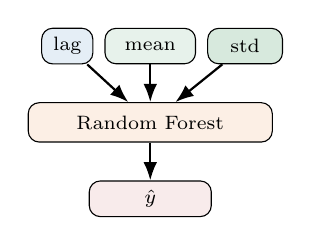
\begin{tikzpicture}[node distance=0.28cm, every node/.style={font=\scriptsize}]
  \node[draw,rounded corners,fill=softblue!15,minimum width=0.65cm,minimum height=0.45cm] (lag) {lag};
  \node[draw,rounded corners,fill=softgreen!15,right=0.14cm of lag,minimum width=1.15cm,minimum height=0.45cm] (mean) {mean};
  \node[draw,rounded corners,fill=softgreen!25,right=0.14cm of mean,minimum width=0.95cm,minimum height=0.45cm] (std) {std};
  \node[draw,rounded corners,fill=softorange!15,below=0.48cm of mean,minimum width=3.1cm,minimum height=0.5cm] (rf2) {Random Forest};
  \node[draw,rounded corners,fill=softred!12,below=0.48cm of rf2,minimum width=1.55cm,minimum height=0.45cm] (pred2) {$\hat y$};
  \draw[-Latex,thick] (lag) -- (rf2); \draw[-Latex,thick] (mean) -- (rf2); \draw[-Latex,thick] (std) -- (rf2); \draw[-Latex,thick] (rf2) -- (pred2);
\end{tikzpicture}
\vspace{0.12cm}

\begin{center}
\begin{tikzpicture}[every node/.style={font=\scriptsize}];
\end{tikzpicture}
\begin{tabular}{rrrr}
\toprule
RMSE & MAE & MAPE & Acc.\\
\midrule
3.23 & 2.12 & 7.29 & 92.71\\
\bottomrule
\end{tabular}
\end{center}
\end{column}
\end{columns}
\vspace{0.05cm}
\centering

\end{frame}
\begin{frame}{Random Forest modellek összehasonlítása}

\vspace{-0.2cm}

\begin{columns}[T,onlytextwidth]

\begin{column}{0.33\textwidth}
\centering
\includegraphics[
  height=0.42\textheight,
  trim=0.4cm 0.4cm 0.3cm 1.5cm,
  clip
]{lagged_predicted_heatmap.png}

{\scriptsize RF lag -- előrejelzés}
\end{column}

\begin{column}{0.33\textwidth}
\centering
\includegraphics[
  height=0.42\textheight,
  trim=0.4cm 0.4cm 0.3cm 1.5cm,
  clip
]{gbm_actual_heatmap_2.png}

{\scriptsize Valós adatok}
\end{column}

\begin{column}{0.33\textwidth}
\centering
\includegraphics[
  height=0.42\textheight,
  trim=0.4cm 0.4cm 0.3cm 1.5cm,
  clip
]{rollingmean_predicted_heatmap.png}

{\scriptsize RF rolling -- előrejelzés}
\end{column}

\end{columns}

\vspace{0.35cm}

\begin{center}
\begin{minipage}{0.8\textwidth}
\begin{block}{Megfigyelés}
A két modell előrejelzése a főbb térbeli mintázatokat jól követi, azonban a rolling feature-ökkel kiegészített modell összességében pontosabb eredményt adott.
\end{block}
\end{minipage}
\end{center}

\end{frame}



% 8
\begin{frame}{Modellek összehasonlítása}

\begin{columns}[T,onlytextwidth]

% BAL OLDAL
\begin{column}{0.62\textwidth}

\begin{table}
\centering
\small
\begin{tabular}{lrrrr}
\toprule
Modell & RMSE & MAE & MAPE & Acc.\\
\midrule
RF rolling & 3.23 & 2.12 & 7.29 & 92.71\\
Baseline & 3.19 & 2.51 & 8.81 & 91.19\\
GBM & 3.34 & 2.64 & 8.93 & 91.07\\
RF lag & 3.11 & 2.53 & 9.18 & 90.82\\
\bottomrule
\end{tabular}
\end{table}

\vspace{0.25cm}

\centering
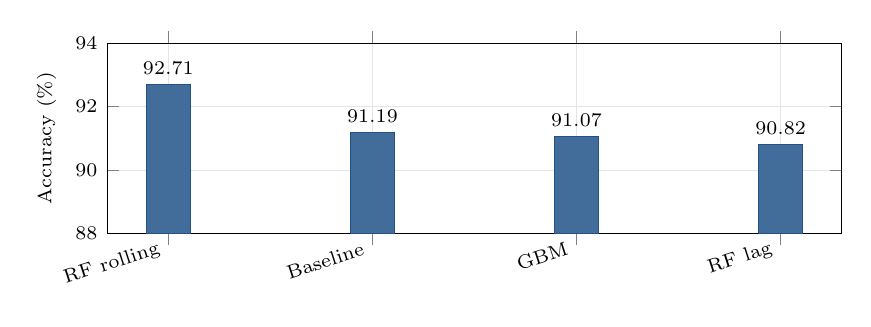
\begin{tikzpicture}
\begin{axis}[
  ybar,
  width=0.9\textwidth,
  height=4.0cm,
  ymin=88,
  ymax=94,
  ylabel={Accuracy (\%)},
  symbolic x coords={RF rolling,Baseline,GBM,RF lag},
  xtick=data,
  xticklabel style={font=\scriptsize,rotate=18,anchor=east},
  tick label style={font=\scriptsize},
  label style={font=\scriptsize},
  nodes near coords,
  every node near coord/.append style={font=\scriptsize},
  bar width=16pt,
  grid=major,
  grid style={gray!20},
]
\addplot[fill=deepblue!85,draw=deepblue] coordinates {
  (RF rolling,92.71)
  (Baseline,91.19)
  (GBM,91.07)
  (RF lag,90.82)
};
\end{axis}
\end{tikzpicture}

\end{column}

% JOBB OLDAL
\begin{column}{0.34\textwidth}

\vspace{0.3cm}

\begin{block}{Fő eredmény}
\centering
\textbf{RF rolling}\\
adta a legjobb relatív pontosságot.
\end{block}

\vspace{0.35cm}

\begin{block}{Értelmezés}
\centering
A rolling feature-ök jobban megragadták a rövid távú mintázatokat.
\end{block}

\end{column}

\end{columns}

\end{frame}

% 9
\begin{frame}{Demográfiai elemzés: másik megközelítés}
\begin{columns}[T]
\begin{column}{0.55\textwidth}
\centering
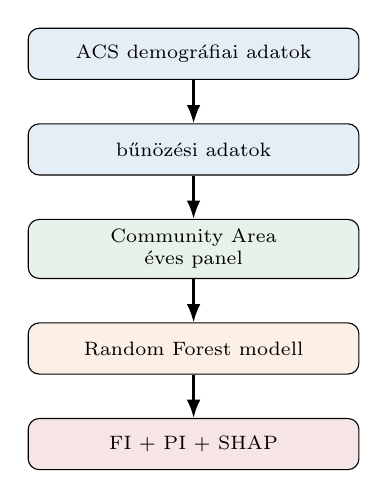
\begin{tikzpicture}[node distance=0.55cm, every node/.style={font=\scriptsize}]
  \node[draw,rounded corners,fill=softblue!15,minimum width=4.2cm,minimum height=0.65cm] (acs) {ACS demográfiai adatok};
  \node[draw,rounded corners,fill=softblue!15,below=of acs,minimum width=4.2cm,minimum height=0.65cm] (crime) {bűnözési adatok};
  \node[draw,rounded corners,fill=softgreen!15,below=of crime,minimum width=4.2cm,minimum height=0.75cm,align=center] (merge) {Community Area\\éves panel};
  \node[draw,rounded corners,fill=softorange!15,below=of merge,minimum width=4.2cm,minimum height=0.65cm] (model) {Random Forest modell};
  \node[draw,rounded corners,fill=softred!15,below=of model,minimum width=4.2cm,minimum height=0.65cm] (interpret) {FI + PI + SHAP};
  \foreach \a/\b in {acs/crime,crime/merge,merge/model,model/interpret}{\draw[-Latex,thick] (\a) -- (\b);} 
\end{tikzpicture}
\end{column}
\begin{column}{0.41\textwidth}
\begin{block}{Itt a cél nem csak predikció}
Mely társadalmi-demográfiai jellemzők hordoznak információt az előrejelzéshez?
\end{block}
\vspace{0.2cm}
\begin{itemize}
  \item népesség,
  \item szegénységi ráta,
  \item jövedelem,
  \item munkanélküliség,
  \item iskolázottság,
  \item fiatal férfiak aránya.
\end{itemize}
\end{column}
\end{columns}
\end{frame}

% 10
\begin{frame}{Példa: Lopás modell -- feature importance és permutation importance}

\begin{columns}[T,onlytextwidth]

\begin{column}{0.49\textwidth}
\centering
\includegraphics[
  width=\textwidth,
  trim=0.2cm 0.2cm 0.2cm 0.2cm,
  clip
]{RF_2024_by_THEFT_szocdem_Feature_importance.png}

{\scriptsize Feature importance}
\end{column}

\begin{column}{0.49\textwidth}
\centering
\includegraphics[
  width=\textwidth,
  trim=0.2cm 0.2cm 0.2cm 0.2cm,
  clip
]{RF_2024_by_THEFT_szocdem_permutation_importance.png}

{\scriptsize Permutation importance}
\end{column}

\end{columns}

\vspace{0.15cm}

\begin{block}{Értelmezés}
Mindkét módszer szerint a \textbf{15--34 éves férfiak aránya} és a \textbf{teljes népesség} kiemelten fontos változó a lopások előrejelzésében.
\end{block}

\end{frame}

% 11



\begin{frame}{Példa: Lopás modell -- SHAP összefoglaló ábra}

\begin{columns}[T,onlytextwidth]

\begin{column}{0.62\textwidth}
\centering
\includegraphics[
  width=0.9\textwidth,
  trim=0.2cm 0.2cm 0.2cm 0.2cm,
  clip
]{RF_2024_by_THEFT_szocdem_shap_summary.png}
\end{column}

\begin{column}{0.34\textwidth}
\begin{block}{Mit mutat a SHAP?}
\begin{itemize}
  \item a változók \textbf{hatásának irányát} is megmutatja,
  \item a \textbf{pozitív SHAP-érték} növeli a becslést,
  \item a \textbf{negatív SHAP-érték} csökkenti a becslést.
\end{itemize}
\end{block}

\vspace{0.15cm}

\end{column}

\end{columns}

\end{frame}

% 12
\begin{frame}{Összesített hőtérkép a leggyakoribb bűncselekménytípusokra}

\begin{columns}[T,onlytextwidth]

\begin{column}{0.72\textwidth}
\centering
\includegraphics[
  width=\textwidth,
  trim=0.2cm 0.2cm 0.2cm 0.2cm,
  clip
]{socio_feature_relative_importance_heatmap_2.png}
\end{column}

\begin{column}{0.25\textwidth}
\begin{block}{Meghatározó változók}
\begin{itemize}
  \item Teljes népesség
  \item Szegénységi ráta
  \item 15-34 éves férfiak aránya
\end{itemize}
\end{block}
\end{column}

\end{columns}

\end{frame}

% 13
\begin{frame}{Következtetések}
\begin{columns}[T]
\begin{column}{0.55\textwidth}
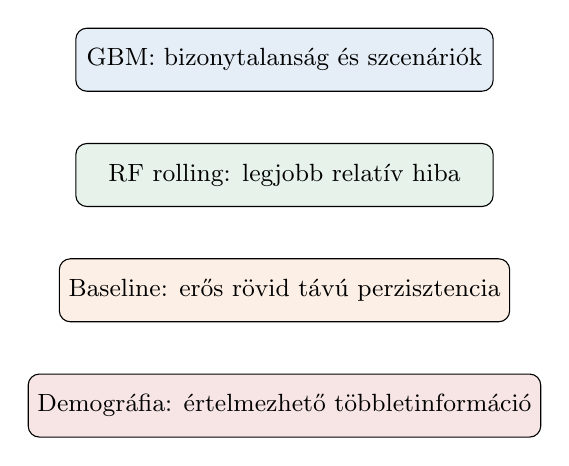
\begin{tikzpicture}[node distance=0.65cm, every node/.style={font=\small}]
  \node[draw,rounded corners,fill=softblue!15,minimum width=5.3cm,minimum height=0.8cm] (c1) {GBM: bizonytalanság és szcenáriók};
  \node[draw,rounded corners,fill=softgreen!15,below=of c1,minimum width=5.3cm,minimum height=0.8cm] (c2) {RF rolling: legjobb relatív hiba};
  \node[draw,rounded corners,fill=softorange!15,below=of c2,minimum width=5.3cm,minimum height=0.8cm] (c3) {Baseline: erős rövid távú perzisztencia};
  \node[draw,rounded corners,fill=softred!15,below=of c3,minimum width=5.3cm,minimum height=0.8cm] (c4) {Demográfia: értelmezhető többletinformáció};
\end{tikzpicture}
\end{column}
\begin{column}{0.4\textwidth}
\begin{block}{Fő üzenet}
A bűnözési gyakoriság több szemlélettel vizsgálható: idősoros, sztochasztikus és társadalmi-demográfiai irányból.
\end{block}
\vspace{0.15cm}
\begin{block}{Módszertani tanulság}
A predikció és az értelmezhetőség eltérő modellezési döntéseket igényel.
\end{block}
\end{column}
\end{columns}
\end{frame}

% 14
\begin{frame}{Köszönöm a figyelmet!}
\centering
\vspace{1.0cm}
{\Large Köszöm a figyelmet!}

\end{frame}

\end{document}
